\documentclass[letterpaper,12pt]{article}
\usepackage{lipsum}  
\usepackage{graphicx}
\usepackage{subcaption}
\usepackage[english]{babel}
\usepackage{fancyhdr}
\usepackage{multicol}

\graphicspath {{figures/}}

\setlength{\headheight}{15pt}

\pagestyle{fancy}
\fancyhf{}
\lhead{\textbf{Version:} 2.0 }% \textbf{Revision:} 05/22/2018}
\rhead{\thepage}
\lfoot{Sam Penders}
\rfoot{\textit{Mu2e: University of Minnesota}}

\renewcommand{\footrulewidth}{1pt}

\newenvironment{myitemize} %adjust item spacing in lists to make smaller
{ \begin{itemize}
    \setlength{\itemsep}{4pt}
    \setlength{\parskip}{0pt}
    \setlength{\parsep}{0pt}     }
{ \end{itemize}                  } 


\begin{document}
\begin{titlepage}
	\centering
	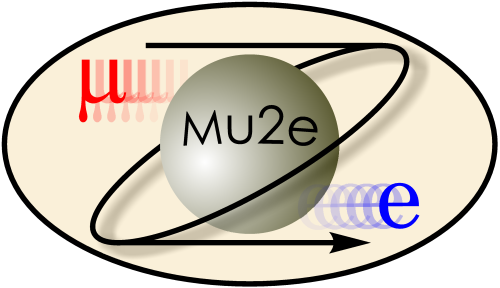
\includegraphics[width=0.5\textwidth]{mu2e_logo_oval.png}\par\vspace{2cm}
	{\scshape\LARGE Making Leak Test\\ Plastic Straw Tubes \\ Version 1.0\par}	\vspace{3cm}
	{\Large Sam Penders\par}
	\vspace{3cm}
	{\large University of Minnesota\par}
 	\vspace{.5cm}
	{\large May 22, 2018\par}
	% Bottom of the page
	\vfill
	{\verb|pende061@physics.umn.edu|\par}
\end{titlepage}

\clearpage
\setcounter{page}{2}


\section{Introduction}
Every straw in the Mu2e tracker is checked for leaks using the leak testing chambers. During these tests, the straws are protected from rubbing against sharp objects by placing them inside of plastic tubes. At the end of the tubes, there is a steel nut attached to a piece of fishing line (Figure \ref{straw tube}). The plastic tubes are extracted from the leak testing chambers by grabbing onto this nut with a magnet.

\begin{figure}[ht]
	\centering
	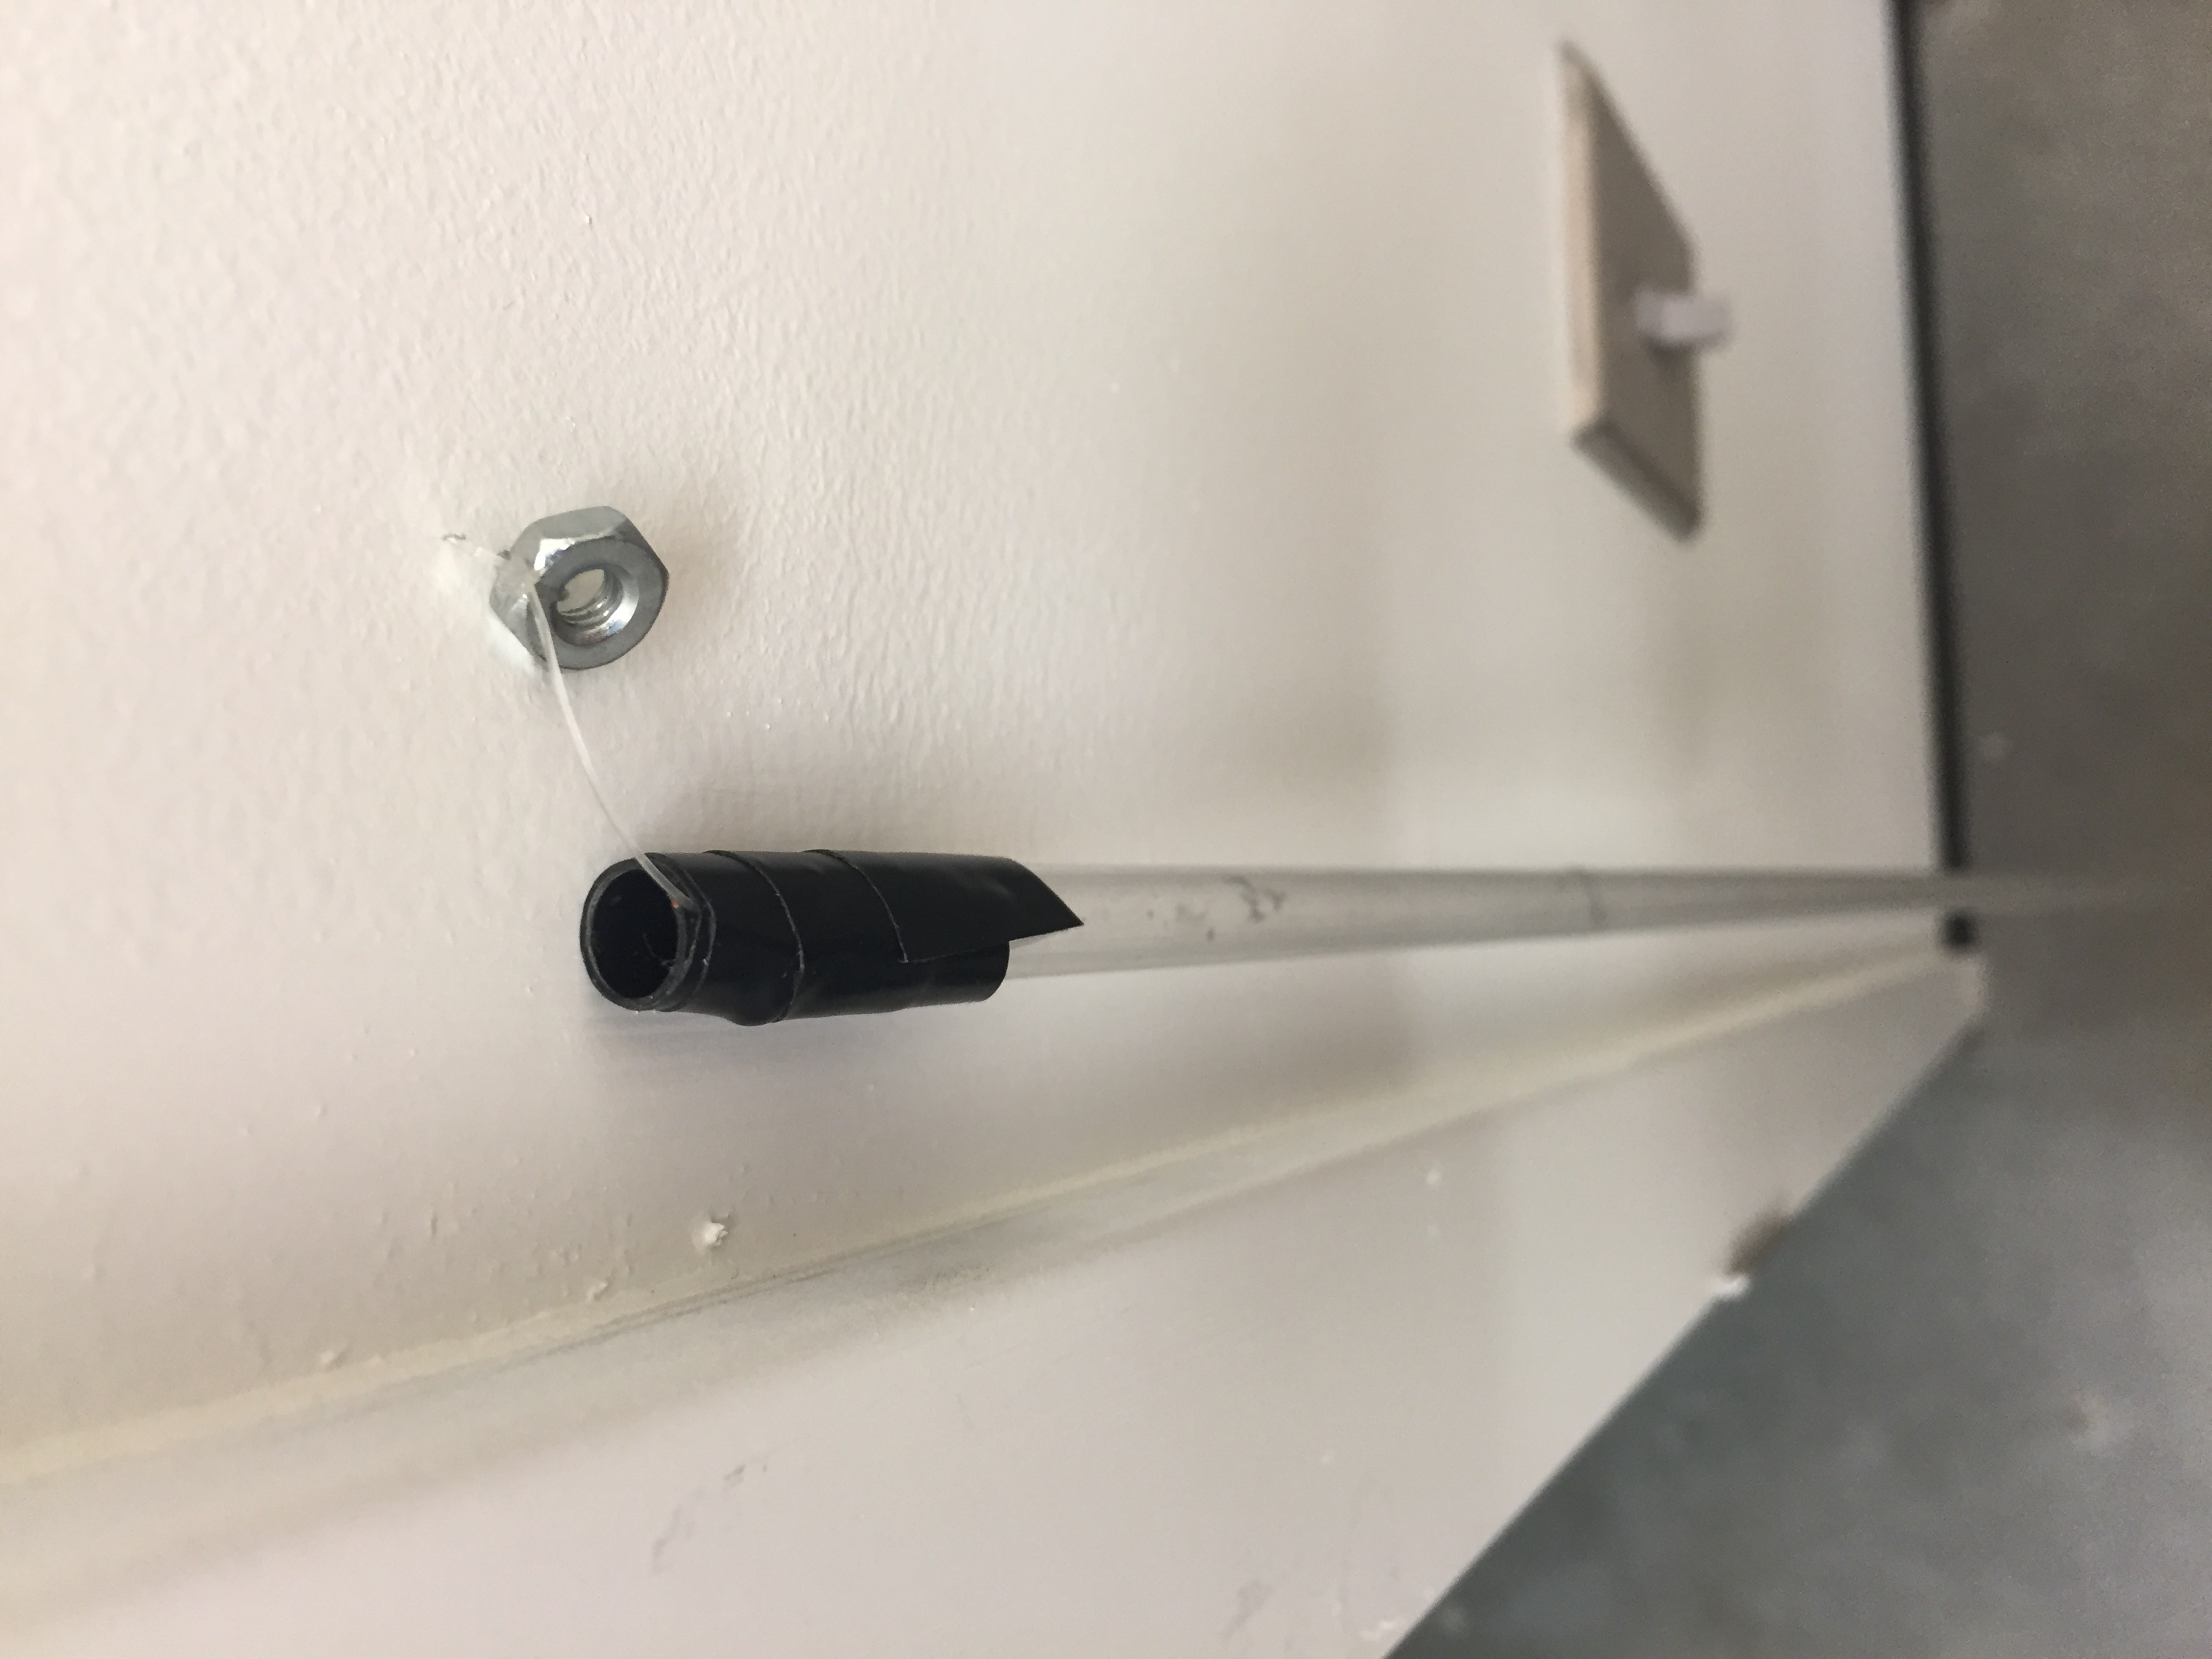
\includegraphics[width=0.7\textwidth, angle=-90]{straw_tube}
	\caption{Plastic tube with steel nut tethered to the end used to protect straws during leak tests.}
	\label{straw tube}
\end{figure}

\newpage

\section{Materials Needed}
	\begin{multicols}{2}
	\begin{myitemize}
		\item Plastic tubes
		\item Nylon fishing line
		\item \#8 hex nuts
		\item Black electrical tape
		\item Scissors
		\item 3M Scotch--Weld DP 100 epoxy
		\item Epoxy mixing nozzle
		\item Epoxy gun
		\item Nitrile gloves	
	\end{myitemize}
	\end{multicols}
	
	\begin{figure}[ht]
		\centering
		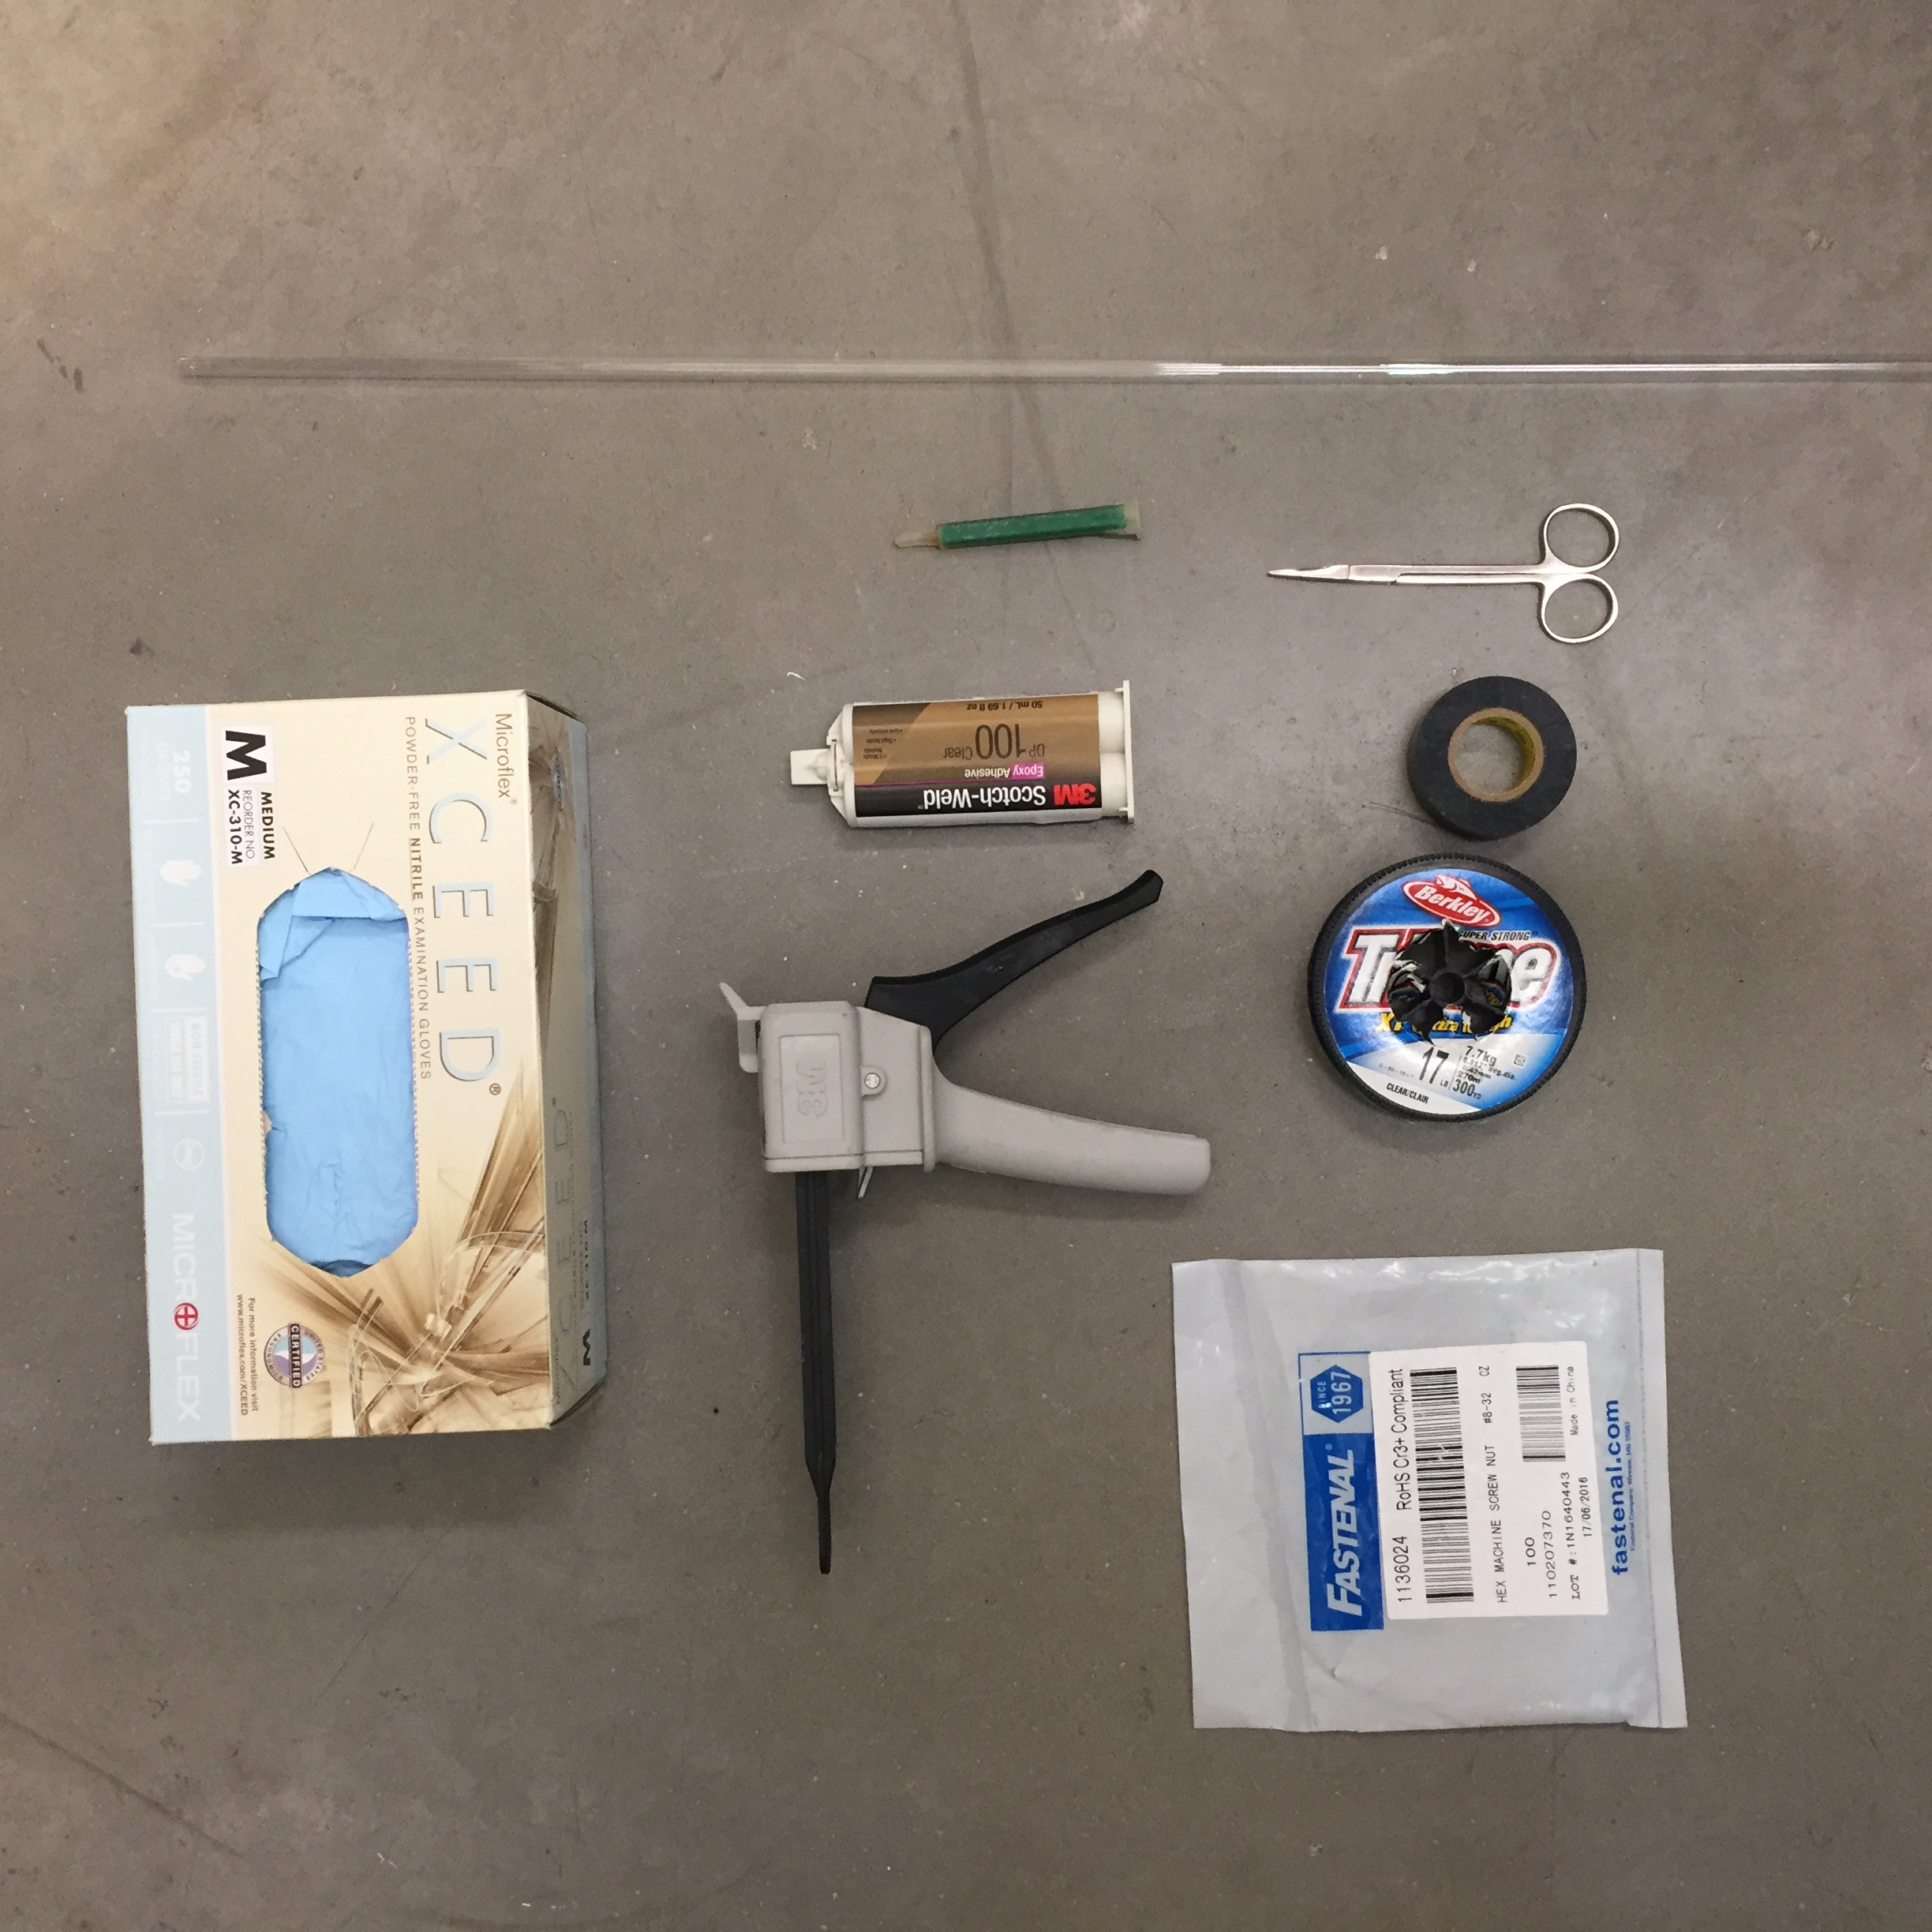
\includegraphics[width=0.7\textwidth, angle=-90]{materials}
	\end{figure}
	
	\newpage
	\section{Risks and Dangers}
3M DP190 epoxy routes of entry, risks, and first aid:
\begin{itemize}
\item {\bf Inhalation:} Remove the person to fresh air. If you feel unwell, seek medical attention.
\item {\bf Skin Contact:} Immediately wash affected area with soap and water. Remove contaminated clothing and wash before reuse. If symptoms develop, seek medical attention.
\item {\bf Eye Contact:} Flush with large amounts of water in eye wash station, located by the main door in PAN 464, and the door without the Ucard reader in room 450. Remove contact lenses is easy to do. If symptoms develop, seek medical attention.
\item {\bf If swallowed:} Rinse mouth. If you feel unwell, get medical attention.
\end{itemize}
	
\newpage
	
\section{Instructions}

\begin{enumerate}
\item Cut off approximately 6 inches of fishing line from the spool.
%
\item With one end of the line, tightly tie a square knot around a \#8 hex nut (Figure \ref{nut square knot}). Figure \ref{square knot} shows how to tie a square knot.
%

\begin{figure}[ht]
	\centering
	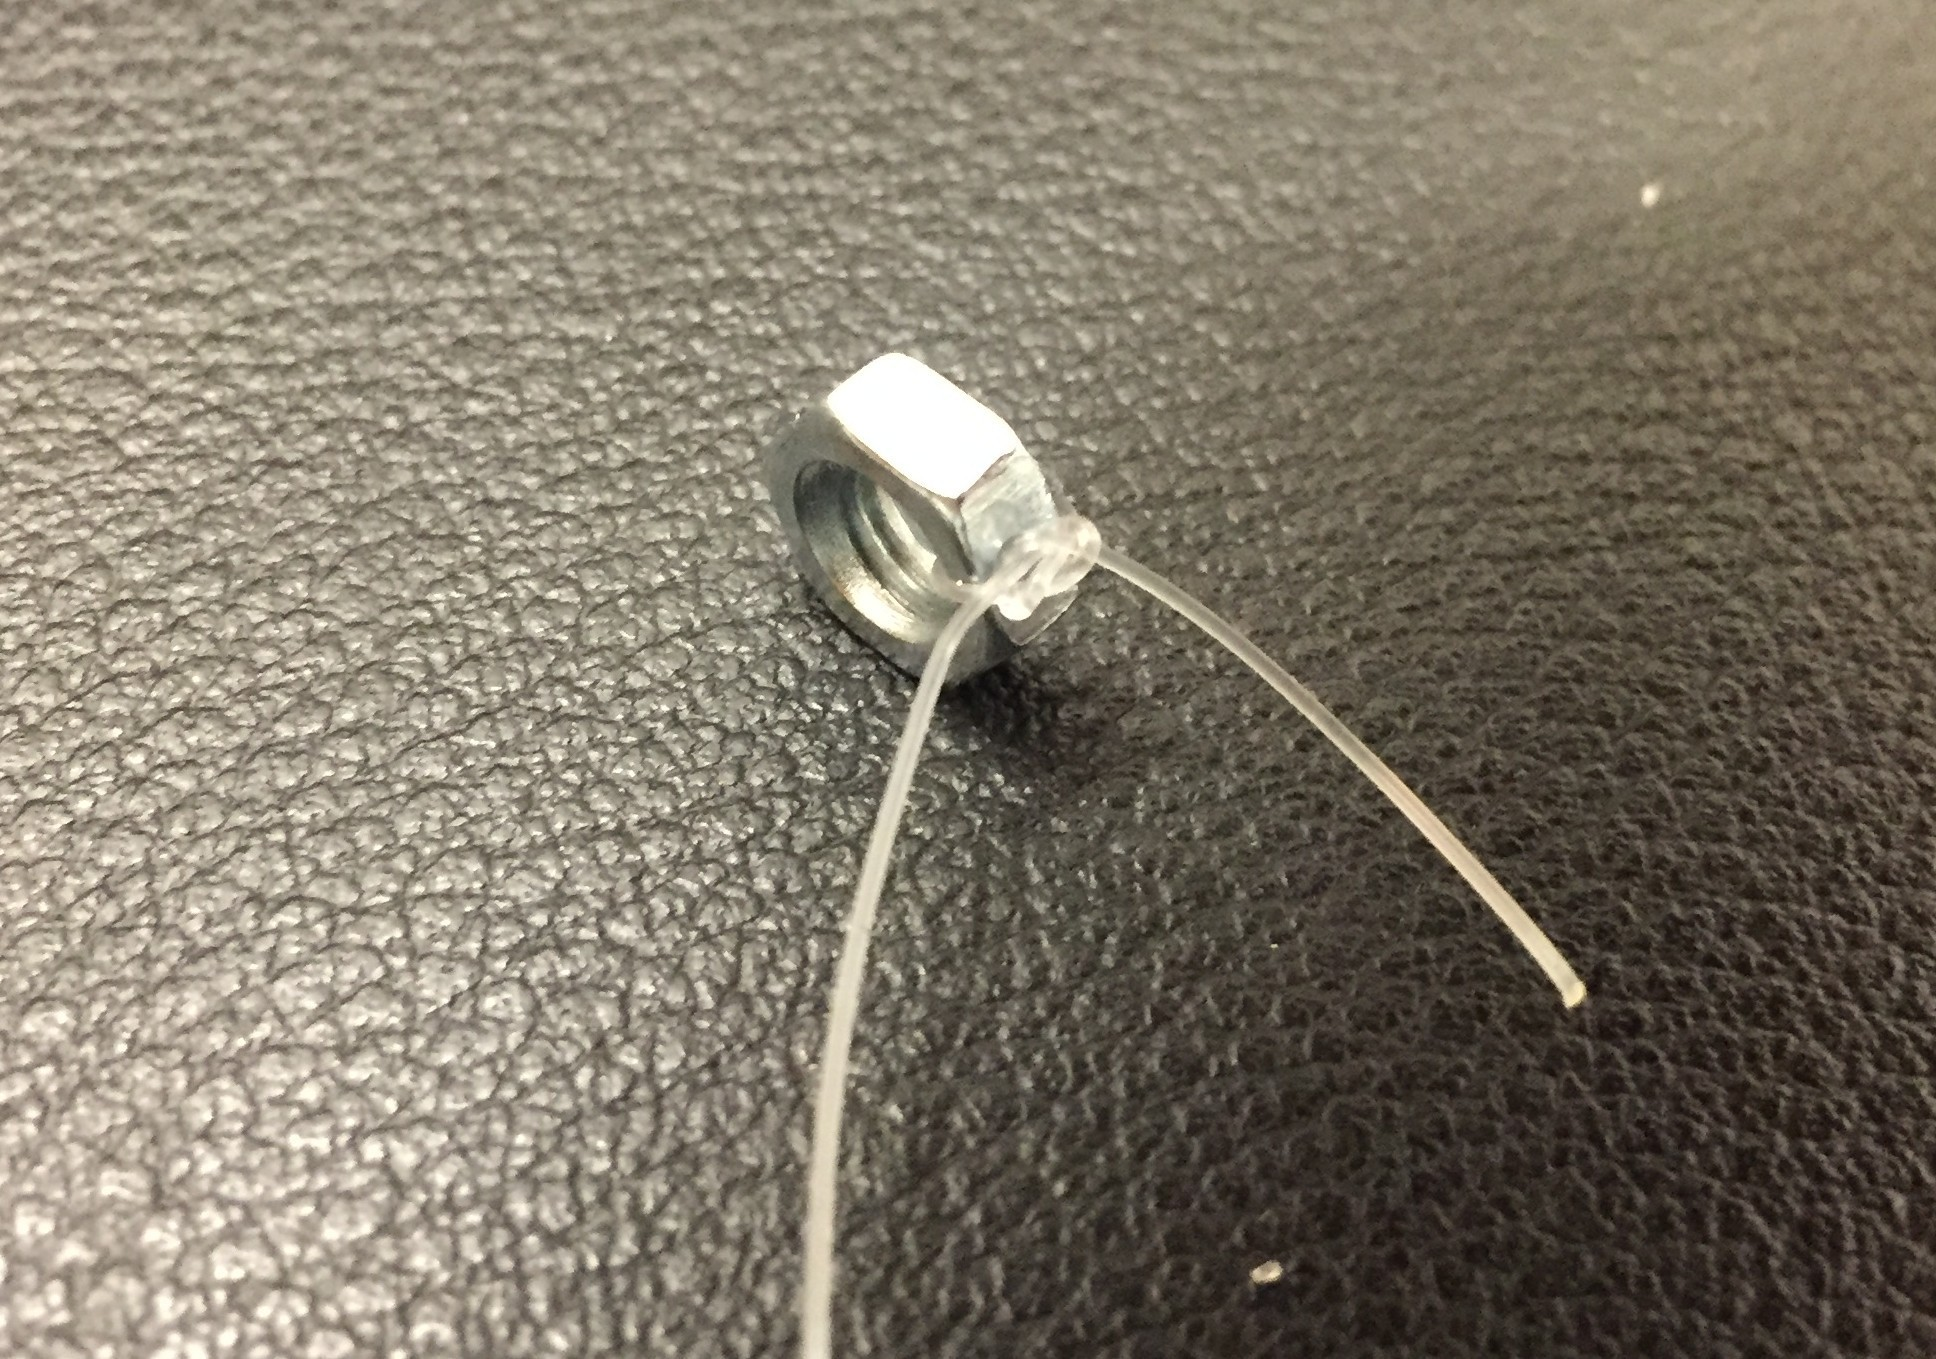
\includegraphics[width=0.6\textwidth]{nut_knot}
	\caption{A square knot tied around a hex nut.}
	\label{nut square knot}
\end{figure}

\begin{figure}[ht]
	\centering
	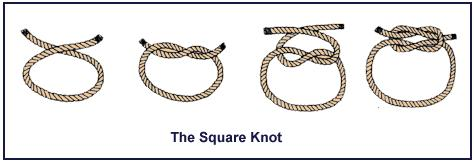
\includegraphics[width=0.8\textwidth]{square_knot}
	\caption{How to tie a square knot. The nut in these instructions should be threaded through the loop in the bottom of the knot.}
	\label{square knot}
\end{figure}


\item Lay the other end of the line against a plastic tube so that the nut is about 1.5 inches from the end of the tube. Tape the fishing line to the tube at two points, leaving a segment of the line exposed (Figure \ref{epoxy tube}). %figure

\begin{figure}[ht]
	\centering	
	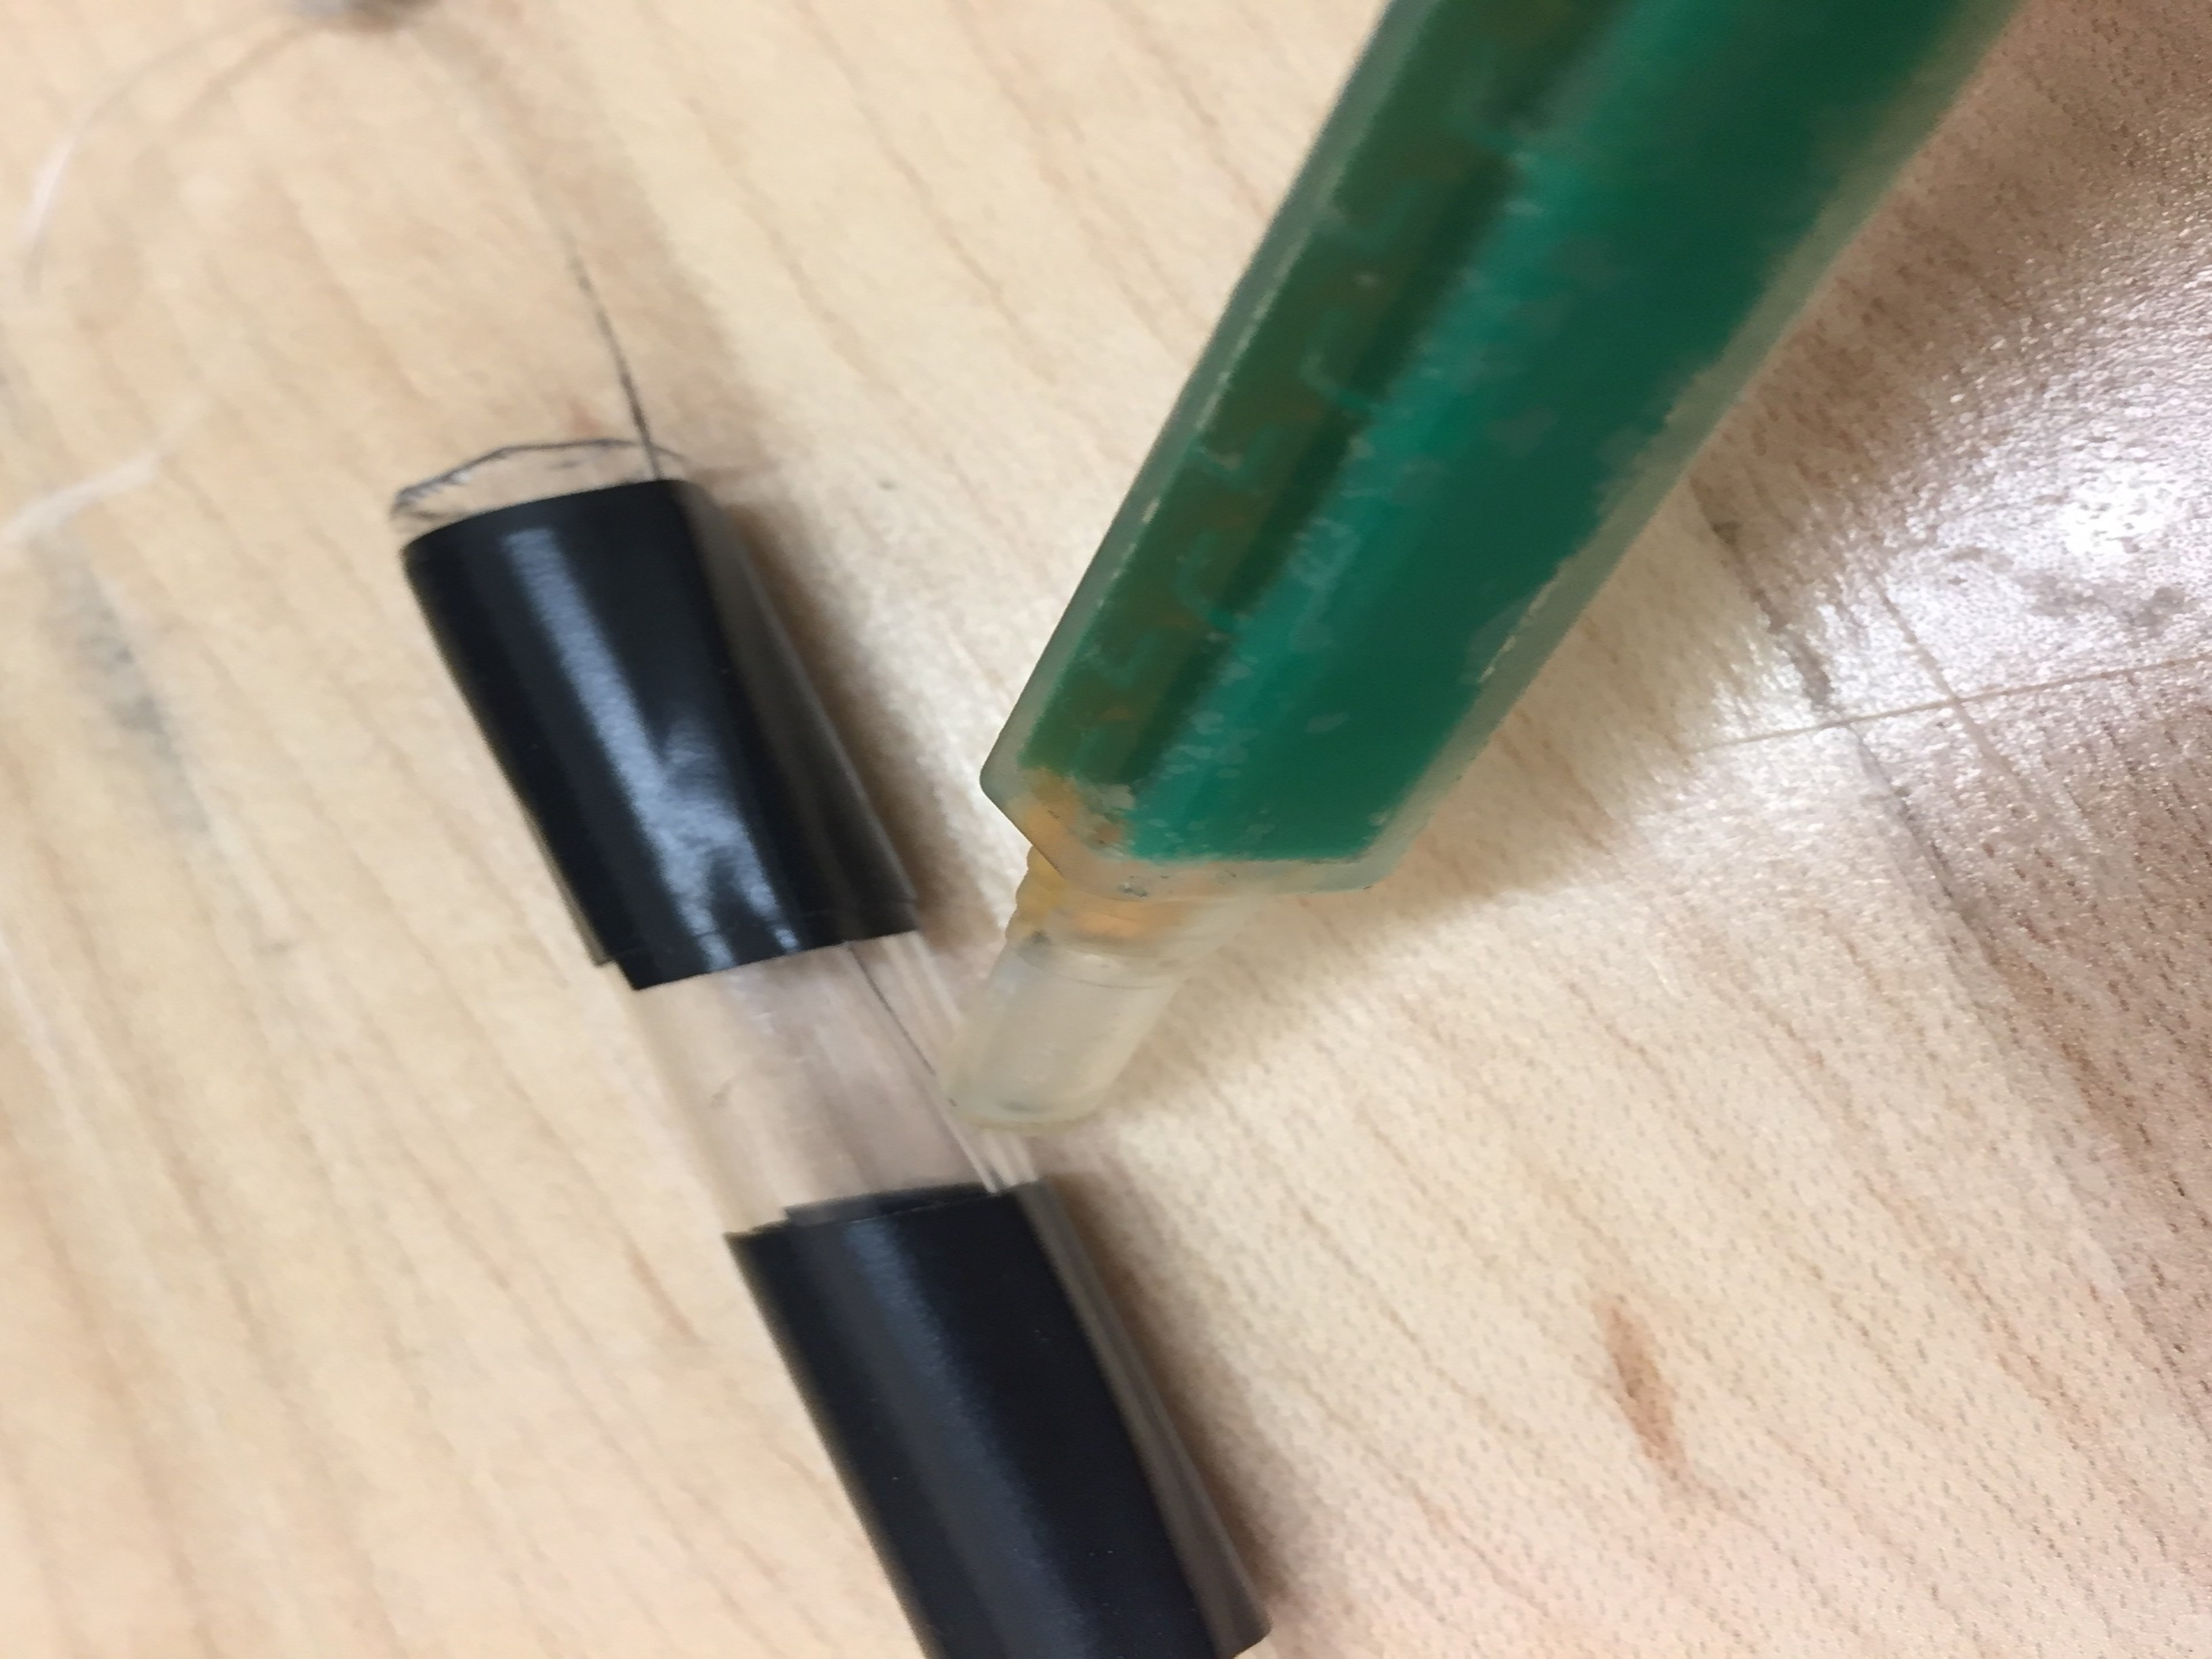
\includegraphics[width=0.45\textwidth]{epoxy_tube}
	\caption{The fishing line is placed against the plastic tube and taped at two sections. In between these two sections, the exposed fishing line gets epoxied.}
	\label{epoxy tube}
\end{figure}
%
\item With the mixing nozzle on the epoxy gun and the epoxy cartridge installed, put a dab of epoxy on the knot around the nut. Also epoxy the fishing line to the plastic tube on the exposed area (Figures \ref{epoxy tube} and \ref{epoxy nut}).


\begin{figure}
	\centering
	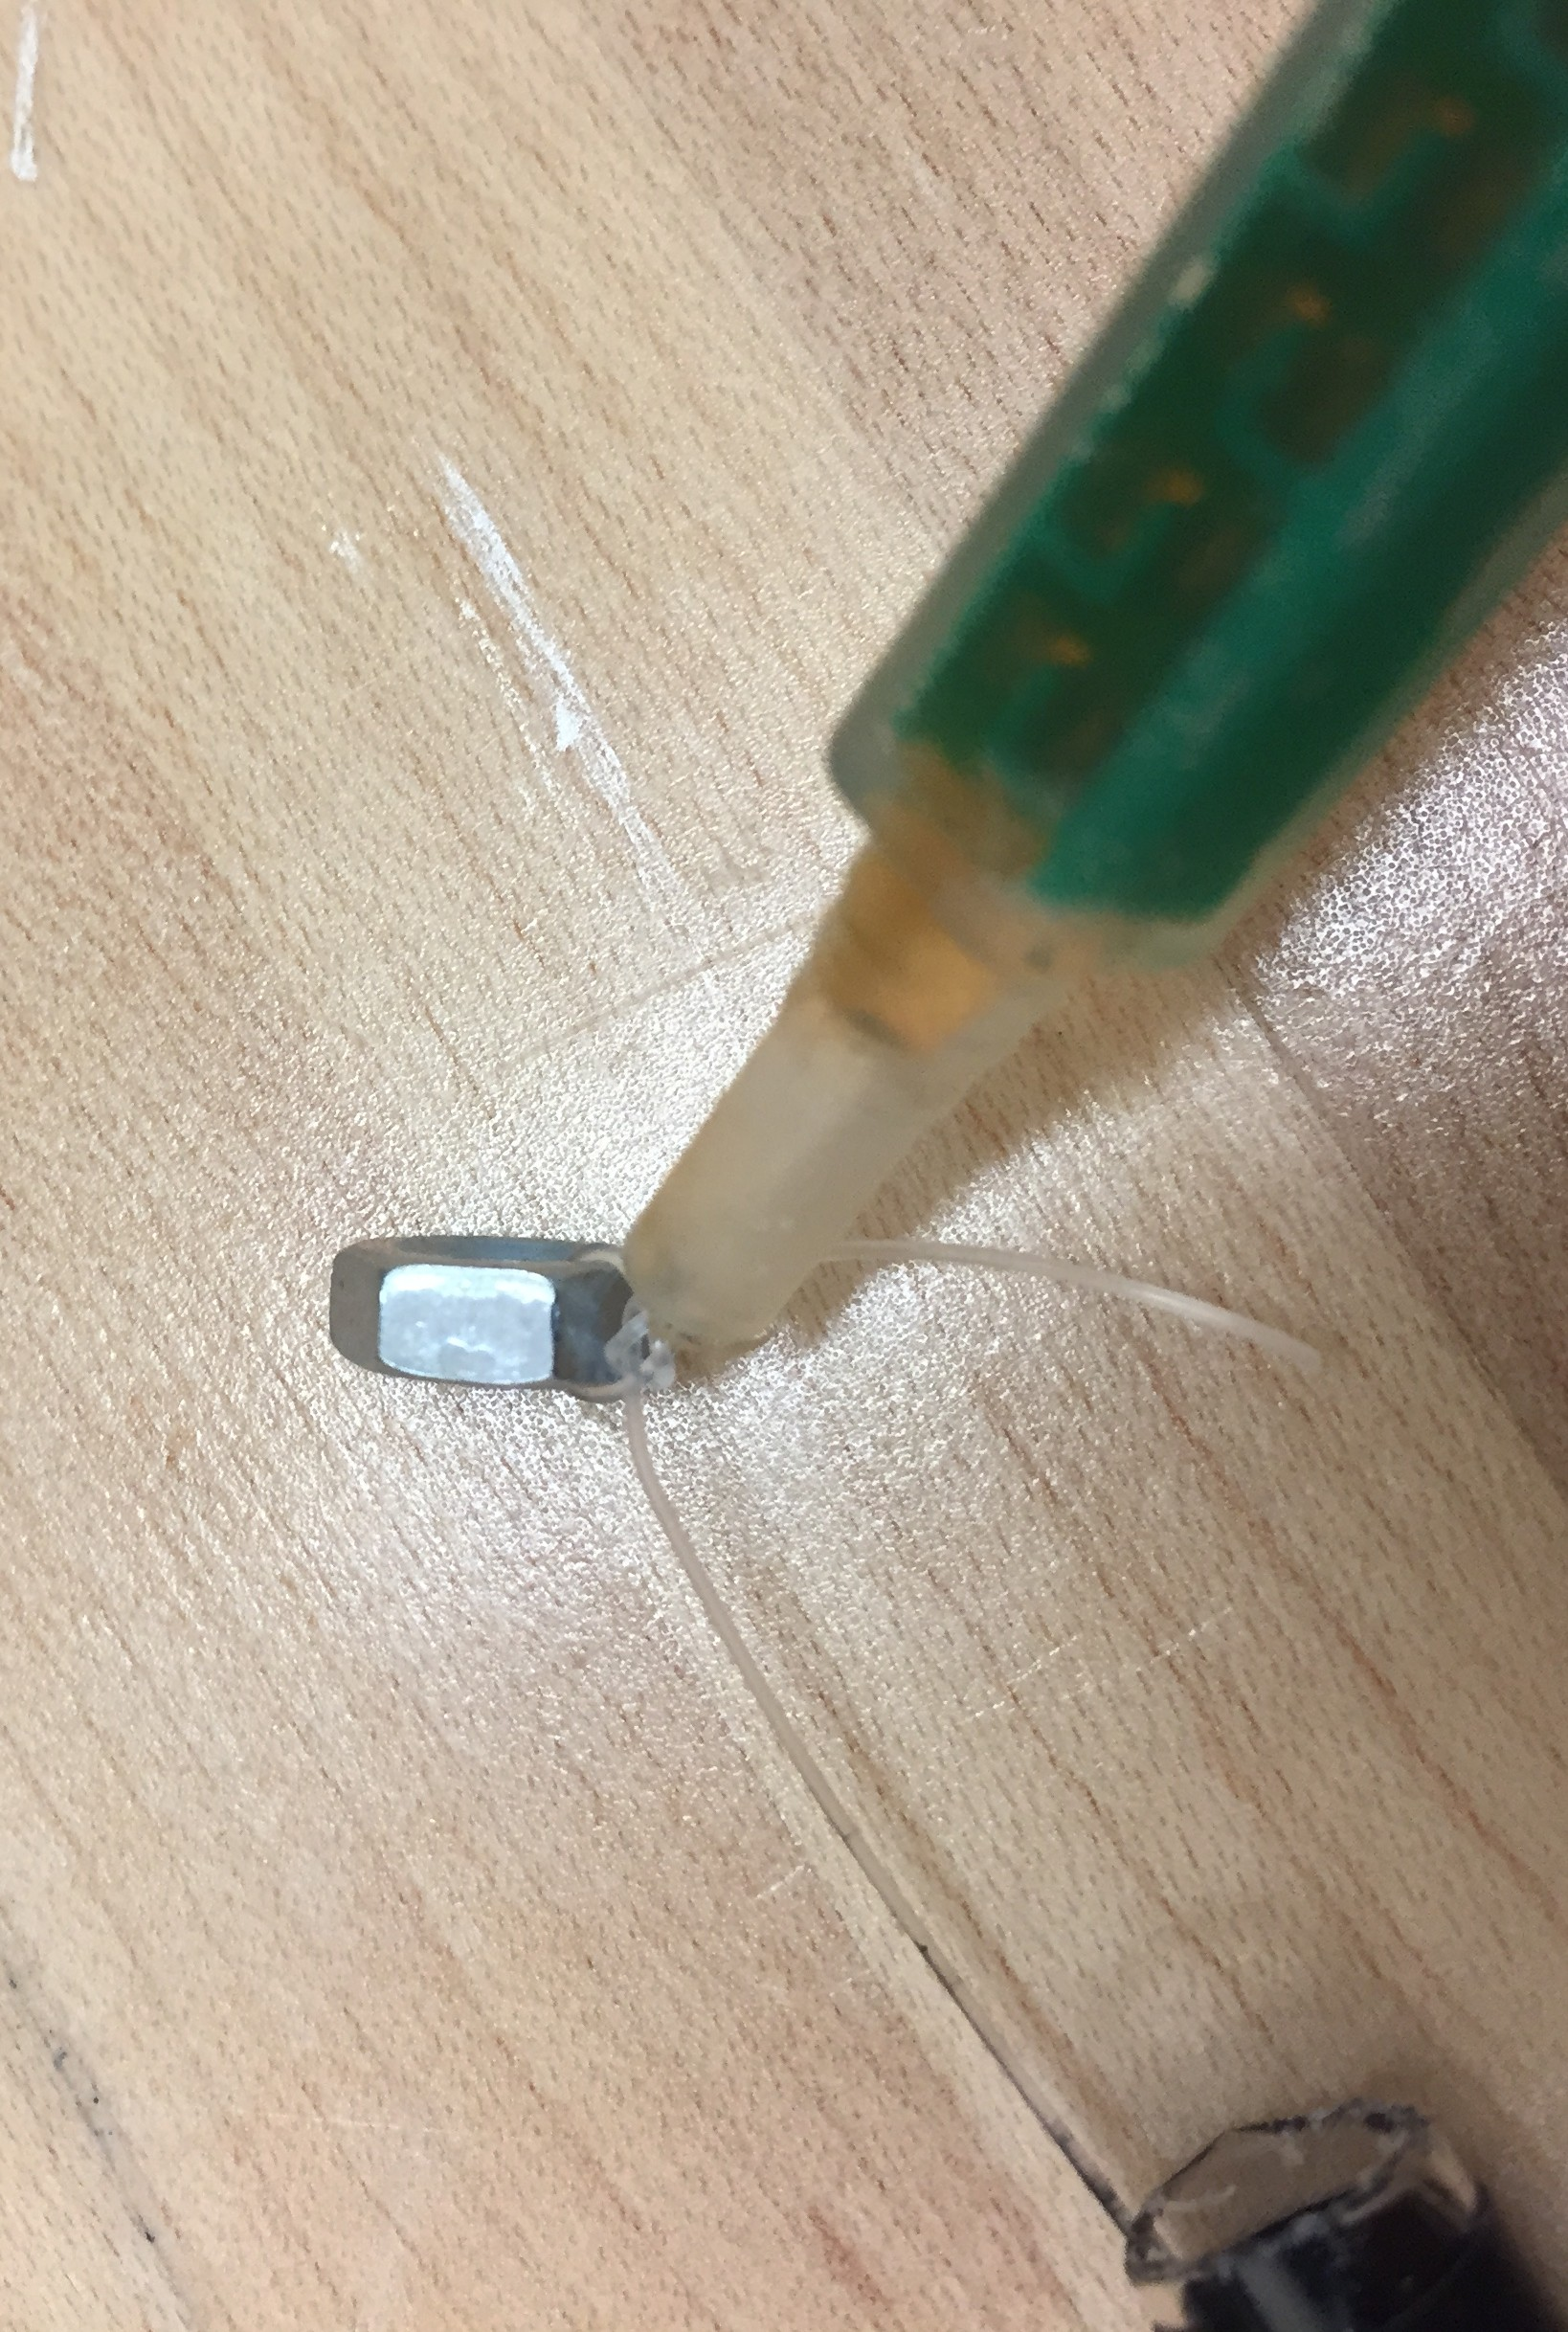
\includegraphics[width=0.3\textwidth, angle=-90]{epoxy_nut}
	\caption{The knot on the nut gets a dab of epoxy applied via the epoxy gun.}
	\label{epoxy nut}
\end{figure}

%
\item Lay the tube down so that the epoxy does not touch any surface, and allow it to cure overnight.

\item Once the epoxy has hardened, wrap electrical tape several times around the epoxied area of the tube, and the area that was already taped. {\bf Note:} the taped area must be thin enough to easily fit into the leak test chambers. Look at completed tubes to get a feel of how thick this is.

\item Check that the epoxy on the nut will secure the knot sufficiently. Cut off any excess fishing line from near the nut, as well as after the taped segment of the tube. The tube should now look like the example in Figure \ref{straw tube}.
\end{enumerate}



\end{document}